% compiler: lualatex
% Preamble
\documentclass[DIV=13]{scrartcl}

% Packages
\usepackage{fontspec}
\usepackage[english]{babel}
\usepackage{amsmath}
\usepackage{amssymb}
\usepackage{tabularray}
\UseTblrLibrary{booktabs}
\usepackage{siunitx}
\usepackage{tabu}
\usepackage{graphicx}
\usepackage[expansion=false]{microtype}
\usepackage[sorting=none, maxbibnames=99, maxcitenames=2,backend=biber]{biblatex}
\usepackage{subcaption}
\usepackage[hidelinks]{hyperref}
\usepackage{csquotes}

\addbibresource{refs.bib}
\usepackage{symbols}

\setmainfont{Tempora}

% Document
\begin{document}
    \title{Rolling Process Variation Estimation Using a Monte-Carlo Method}
    \date{\today}
    \author{%
        M.~Weiner \thanks{Corresponding author}
        \and
        C.~Renzing
        \and
        J.~Mantel
        \and
        M.~Schmidtchen
        \and
        U.~Prahl
    }

    \extratitle{%
        \minisec{Max Weiner}
        max.weiner@imf.tu-freiberg.de\\
        Conceptualization, Methodology, Software, Formal analysis, Validation, Investigation, Writing - Original Draft\\
        Institute of Metals Forming, TU Bergakademie Freiberg

        \minisec{Christoph Renzing}
        christoph.renzing@imf.tu-freiberg.de\\
        Software, Validation, Investigation, Project administration, Writing - Review \& Editing\\
        Institute of Metals Forming, TU Bergakademie Freiberg

        \minisec{Jennifer Mantel}
        jennifer.mantel@imf.tu-freiberg.de\\
        Writing - Review \& Editing, Data curation\\
        Institute of Metals Forming, TU Bergakademie Freiberg

        \minisec{Matthias Schmidtchen}
        matthias.schmidtchen@imf.tu-freiberg.de\\
        Conceptualization, Supervision, Resources, Project administration, Writing - Review \& Editing\\
        Institute of Metals Forming, TU Bergakademie Freiberg

        \minisec{Ulrich Prahl}
        ulrich.prahl@imf.tu-freiberg.de\\
        Supervision, Resources, Writing - Review \& Editing\\
        Institute of Metals Forming, TU Bergakademie Freiberg

        \vfill

        \minisec{Funding}
        Not applicable.

        \minisec{Data Availability}
        Data openly available in a public repository that does not issue DOIs.
        Source code and data are available on GitHub at the following URLs:
        \begin{description}
            \item[Project Home] \url{https://github.com/pyroll-project}
            \item[Core Package] \url{https://github.com/pyroll-project/pyroll-core}
            \item[Benchmark Input and Data] \url{https://github.com/pyroll-project/pyroll-pub1-benchmark}
        \end{description}

        \minisec{Conflicts of Interest}
        The authors declare no conflicts of interest.

        \minisec{Acknowledgements}
        The authors thank Richard Pfeifer and Lukas Göschel for the preparation of the data.

        \minisec{Keywords}
        Rolling Simulation; Open Source; Groove Rolling
    }

    \maketitle

    \begin{abstract}
        Industrial processes are subject to uncertainties originating in variations of input material and process parameters,
        especially if manual treatment is involved.
        For hot rolling processes, in particular,
        variations in workpiece geometry and temperature are affecting the final product shape and material properties.
        In this work, a Monte-Carlo-Method is applied to a fast hot rolling model based on the open-source rolling simulation framework PyRolL for estimating and analysing the variational behaviour of an experimental semi-continuous rolling line for steel wire production.
        The effects of input tolerances and manual transport between the reversing passes on the final product properties are quantified.
        Crucial stages of the process in regard to product properties are identified
        The findings are compared with practical knowledge and experimental results of statistical rolling trials.
    \end{abstract}


    \section{Introduction}\label{sec:introduction}

    All technical processes are subject to certain variations.
Knowledge and control of these variations is crucial for process stability and product quality.
Sources of variations in a process are the variations already present in the input workpiece,
like geometry, chemical composition, microstructural state and temperature distribution,
as well as newly generated variations due to imperfections of the process itself.
In the case of wire and bar hot rolling industry regarded here, not only the product geometry, but also the final material properties are highly sensitive to the process conditions.
Especially the temperature evolution of the workpiece within the rolling train has high impact on the microstructural transformation processes happening before, during and after forming.
The product's microstructural state determines the mechanical properties and therefore its behaviour in further processing and application.
Current alloy concepts in the steel industry increase this problem, as the process window gets more narrow to achieve the property requirements for high-tech applications.
The controlled combination of forming and thermally activated material transformation is commonly subsumed under the term thermo-mechanical treatment.

The classic way of analysing variational behaviour with mathematical tooling is the error propagation using first order Taylor series expansions (see f.e.~\cite{Ku1966}).
This concept is widely used in science and industry, especially to determine the error of indirect measurement processes.
This procedure has two main problems.
First, one needs to determine the first derivatives of the regarded function in each dimension, either analytically or numerically, which is rather problematic if the function is complicated.
Second, the error is commonly represented in terms of the variance, so there is only information about the spread, but not about the shape of the distribution inherent.

The usage of a Monte-Carlo Method circumvents these problems, and shall be proposed with this work.
The term Monte Carlo Method (MCM) generally refers to a class of methods, which are characterized by the use of random numbers.
These methods are rather diverse and serve different purposes.
Here, the term shall be used for the concept of drawing random numbers as input for a function and analysing the results of several evaluations of this function, with different random inputs, with statistical methods.
A detailed overview on this type of Monte Carlo methods is given by \textcite{Lemieux2009}.
The nature of the function can be complicated, even of a black-box type, where nothing about the internals of the function is known but the input and output interfaces.
In this case, Monte Carlo methods can provide valuable information about the behavior of the function while altering inputs.
Also, the complete distribution of the input variables is included in the estimation and is reflected in the results.

Here, the function equals the simulation procedure, so it is generally known, but complicated.
For example, it is generally not possible, to compute derivatives of the outputs in dependence on the inputs in an analytical way.
Even numerical derivation is hard, due to the multi-dimensional nature of most natural or technical systems and the pronounced non-linear behavior of the function.

The use of Monte Carlo methods for the analysis of variations in technical processes was reported before in the field of assembly of complicated structures, like in mechanical engineering and building construction (f.e.~\cite{Lin1997, Shen2005, Dantan2009, Qureshi2012, Yan2015, Rausch2019}).
However, in the field of rolling processes, there was no such attempt yet to the knowledge of the authors.
The authors have previously used a similar approach to model powder morphology influences in sintering processes~\cite{Weiner2022, Weiner2022b}.
The current work shall show the possibility of the application of Monte Carlo methods for the analysis of process variations in rolling processes.
The focus lies hereby on the estimation of the workpiece temperature evolution and its impact on the microstructure state of the final product.
The influence of variations in the initial workpiece and within the regarded process route is analysed and evaluated.
Due to the need of a large number of function evaluations (simulation runs), the evaluation speed of the process model is crucial to the applicability of this approach.

Rolling simulation is currently dominated by the use of finite element (FE) based models (f.e.~\cite{Kim2005, Liu2002, Takashima2014}).
These are offering high accuracy and high resolution results at the expense of high computational resource usage.
So these methods are inconvenient for the current need.
Therefore, one-dimensional semi-analytical approaches shall be used here, as were common in former days, when computer power was not available or a rare resource (f.e.~acc.~to~\textcite{Hensel1978, Wusatowski1969, Lendl1948, Sims1954}).
These offer less accuracy and limited resolution, but are nowadays computable within fractions of seconds on typical personal computer systems.
So these models come to a new shine in enabling the use of numerical routines around the actual simulation core requiring a large number of evaluations, like in optimization or uncertainty analysis.
The simulations are conducted using the open-source rolling simulation framework PyRolL~\cite{pyroll_jors}, developed by the authors, which is a fast, open and flexible software package mainly aimed at groove rolling in elongation passes.
The models used for the different parts of the problem can be exchanged and extended with low effort to the users needs.




    \section{Methods}\label{sec:methods}

    \subsection{Experimental Procedure}\label{subsec:experimental-procedure}

The object of the current investigation is the operation of the experimental semi-continuous rolling plant located at the Institute of Metal Forming, TU Bergakademie Freiberg.
It consists of a two-high reversing roughing stand and four continuous finishing stands.
The pass schedule of the current work consists of 10 oval-round reversing passes followed by 4 oval-round continuous finishing passes.
A \qty{50}{\milli\meter} round workpiece made of C45 carbon steel is rolled down to \qty{8}{\milli\meter} diameter, starting at \qty{1150}{\celsius}, resp.\ \qty{1423.15}{\kelvin}.
Details of the schedule are provided in \autoref{tab:process_conditions} and in the supplemental material~\cite{WeinerVariationSupplemental2023}.
The profile shapes appearing in the schedule are illustrated in \autoref{fig:plot_pass_sequence}.

\begin{figure}
    \centering
    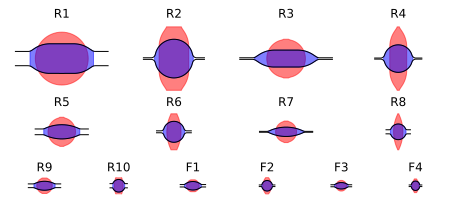
\includegraphics{img/plot_pass_sequence}
    \caption{True Scaled Illustration of the Investigated Pass Sequence}
    \label{fig:plot_pass_sequence}
\end{figure}


\begin{table}
    \centering
    \caption{Principal Data of the Investigated Pass Sequence}
    \label{tab:process_conditions}
    \begin{tblr}{colspec={l|XXXXXX}}
    \toprule
    \#             & Type                       & $\Width$                                               & $\Height$                                              & $\RollGap$                              & $\RollRadius$                                           & $\Velocity$                          \\
    &                            & \unit{\milli\meter}                                    & \unit{\milli\meter}                                    & \unit{\milli\meter}                     & \unit{\milli\meter}     & \unit{\meter\per\second}   \\
    \midrule
    
    {{loop.index}} & {{ p | format_pass_type }} & \num{ {{- (p.out_profile.width * 1e3) | round(1) -}} } & \num{ {{-  (p.out_profile.height * 1e3) | round(1) -}} } & \num{ {{-  (p.gap * 1e3) | round(1) -}} } & \num{ {{-  (p.roll.nominal_radius * 1e3) | round(1) -}} } & \num{ {{-  p.velocity | round(1) -}} }\\
    
    \bottomrule
\end{tblr}
\end{table}

Online measurements of the process conditions and workpiece state are done regarding roll force and torque, as well as workpiece temperature.
The latter is measured using pyrometers at several points in the plant: at entry and exit of the reversing stand and before, between and after the finishing stands.
The sensor signals are collected as timelines, so that they can be automatically analysed afterwards as described in \autoref{subsec:data-acquisition}.

To achieve statistical certainty, a number of 45 rolling trials were carried out.
This enables an estimation of the variations appearing.
A major source of variation in these trials is the manual feeding of the workpiece into the reversing passes.
The duration of those is scheduled with about 6 seconds.
The actual time needed has to be investigated in this work, see \autoref{subsec:data-acquisition} for details.

\subsection{Monte-Carlo Approach}\label{subsec:monte-carlo-approach}

\begin{figure}
    \centering
    \includegraphics[width=\linewidth]{img/chart_mc_principle}
    \caption{Chart of the Concept of Variation Estimation Using Monte Carlo Techniques}
    \label{fig:chart_mc_principle}
\end{figure}

The basic idea of the approach shown here is to simulate the rolling process several times with different input values, which are drawn by a random number generator according to predefined statistical distributions.
Afterwards, the distribution of the results can be analysed by classic methods of descriptive statistics to obtain information about the process' variational behavior.
The principle is shown in \autoref{fig:chart_mc_principle}.

This approach provides information about the overall variational behavior of the process.
If a single source of variation is introduced in the input, the reaction of the process on this variable can be analysed.
The count of variation sources introduced is generally unbounded.
In contrast to classic Taylor series error propagation, the computational effort does not directly increase remarkably with increasing count of investigated parameters.
However, an increase in sample size can be necessary to achieve sufficient certainty.
The key problem is to obtain data describing the variations of the input variables.
The tracing back of result variations to the input can be done using classic correlation methods of descriptive statistics, however, with the same typical caveats.
The main benefit of the approach is, that no information about the internals of the simulation procedure is needed for variational analysis, especially there is no need for derivatives of result values in dependence on the input.
The simulation procedure can generally be treated as black box with defined input and output interfaces.

\subsection{Statistical Data Acquisition}\label{subsec:data-acquisition}

As input for the Monte-Carlo approach statistical descriptions of the regarded input variables are needed.
Regarding the geometric variations of the input workpiece, the diameter of the samples was determined at multiple spots using a calibre.
The initial temperature of the samples was determined using the pyrometer installed near the roll gap entry.
Both were approximated using a normal distribution for sampling of random input values.

The question of varying inter-pass durations is crucial for scientific experiments on microstructure evolution, but currently often neglected.
Mostly, only fixed durations between the reversing passes are included in the design calculations.
Due to manual transport and feed of the workpiece to the following roll pass, the scheduled inter-pass durations are never realized in practice.
Although, these deviations from the schedule influence the microstructure evolution of the sample, as well as the actual conditions in the roll passes.
The current approach is aimed to help quantifying these deviations.

To obtain the inter-pass durations from the timeline data, the passes have to be identified automatically.
This was done by analysing the roll torque signal as plotted in \autoref{fig:plot_timeline_pass_finding}.
The original signal was first downsampled and smoothed.
Then, a difference filter was applied and the peaks of the resulting signal were determined.
These peaks denote start and end times of the roll passes, the middle time of those was used as time coordinate of the roll pass.
The distances of those were used as the inter-pass durations.

\begin{figure}
    \centering
    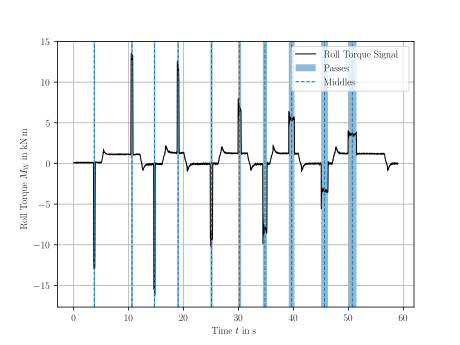
\includegraphics{img/plot_timeline_pass_finding}
    \caption{Example Roll Torque Signal With Automatically Determined Roll Pass Locations}
    \label{fig:plot_timeline_pass_finding}
\end{figure}

For the approximative description of the durations' distribution, a gamma distribution was used, which is a generalized exponential distribution.
The probability density function (PDF) of the gamma distribution is defined as in \autoref{eq:gamma-dist}, where $\Gamma$ is the gamma function and $\GammaDistributionAlpha > 0$ and $\GammaDistributionBeta > 0$ are parameters.

\begin{equation}
    f(x) = \frac{\GammaDistributionBeta^\GammaDistributionAlpha}{\Gamma(\GammaDistributionAlpha)}x^{\GammaDistributionAlpha - 1} \exp(-\GammaDistributionBeta x)
    \label{eq:gamma-dist}
\end{equation}

Since the gamma distribution is only defined for $x>0$, but no inter-pass durations below a certain value occur due to technical restrictions, the distribution was modified by introducing a minimal inter-pass duration $\MinInterpassDuration$ with $x = \InterpassDuration - \MinInterpassDuration$.
So there are three free parameters $\GammaDistributionAlpha$, $\GammaDistributionBeta$ and $\MinInterpassDuration$ for fitting of the distribution function.
The fitting was done using least squares optimization of the PDF function on the density histogram of the data.

\subsection{Core Simulation Procedure}\label{subsec:simulation-procedure}

In the current work, the open-source rolling simulation framework PyRolL~\cite{pyroll2} was used to simulate the rolling process.
Generally, the shown approach can be used with every rolling simulation software available, since the procedure does not depend on any internals of the simulation.
A fast simulation approach, however, is favourable, since the simulation has to be done several, up to hundreds of, times.
The models used here are of one-dimensional type, thus, they lack of resolution in other directions as the rolling direction and provide only limited accuracy, but at the benefit of high solution speed.
They typically combine empirical approaches with simplified analytical solutions.
The simulation was done with the basic configuration of PyRolL, which includes the empirical roll force and torque model of \textcite{Hensel1978}, an integral thermal model approach according to \textcite{Hensel1990}, contact area estimation according to \textcite{Zouhar1960} and roll flattening according to \textcite{Hitchcock1935}.
Spreading was simulated using the equivalent flat pass according to \citeauthor*{Lendl1948}~\cite{Lendl1948, Lendl1948a, Lendl1949} in conjunction with the spreading equation of \textcite{Wusatowski1969}.
Details of software construction and model equations are provided in the documentation of PyRolL~\cite{pyroll}.


% TODO: kurze Beschreibung der wichtigsten Modelle: Thermik, Mikrostruktur, Hensel

The models most important for the following elaborations will be discussed in brief.
The temperature change of the workpiece was calculated by an integral heat balance as proposed by \textcite{Hensel1990} and given in \autoref{eq:heat-balance}.

\begin{equation}
    \Delta\Temperature = \Delta\Temperature_\Convection + \Delta\Temperature_\Contact + \Delta\Temperature_\Deformation + \Delta\Temperature_\Radiation
    \label{eq:heat-balance}
\end{equation}

\noindent$\Delta\Temperature_\Convection$ is the temperature change by convective heat flows according to \autoref{eq:heat-convection} with $\HeatTransferFactor_{\Convection}$ as a heat transfer factor, $\Temperature_\Environment$ as the environment temperature, $\Temperature$ as the current workpiece temperature and $\Time$ as the duration of the process step.

\begin{equation}
    \Delta\Temperature_\Convection = \HeatTransferFactor_{\Convection} \left( \Temperature_\Environment - \Temperature \right) \Time
    \label{eq:heat-convection}
\end{equation}

\noindent$\Delta\Temperature_\Contact$ is the temperature change by contact to the rolls according to \autoref{eq:heat-contact} with $\HeatTransferFactor_{\Contact}$ as a heat transfer factor and $\Temperature_{\Roll}$ as the temperature of the rolls.

\begin{equation}
    \Delta\Temperature_\Contact = \HeatTransferFactor_{\Contact} \left( \Temperature_\Roll - \Temperature \right) \Time
    \label{eq:heat-contact}
\end{equation}

\noindent$\Delta\Temperature_\Radiation$ is the temperature change by radiation according to \autoref{eq:heat-radiation} with $\StefanBoltzmannCoefficient$ as the Stefan's and Boltzmann's constant and $\RelativeRadiationCoefficient$ as the relative radiation coefficient of the gray radiator.

\begin{equation}
    \Delta\Temperature_\Radiation = \StefanBoltzmannCoefficient \RelativeRadiationCoefficient \left( \Temperature_\Environment^4 - \Temperature^4 \right) \Time
    \label{eq:heat-radiation}
\end{equation}

\noindent$\Delta\Temperature_\Deformation$ is the temperature change by deformation according to \autoref{eq:heat-deformation} with $\DeformationResistance$ as the empirical deformation resistance and $\Equivalent\LogStrain$ as the equivalent plastic strain.
Since the deformation resistance is used here instead of the flow stress, this term also includes approximately the heat generation by inner and outer friction.

\begin{equation}
    \Delta\Temperature_\Deformation = \num{0.95} \DeformationResistance \Equivalent\LogStrain
    \label{eq:heat-deformation}
\end{equation}

The deformation resistance was taken as proposed by \textcite{Hensel1978} and given in \autoref{eq:deformation-resistance}.

\begin{multline}
    \frac{\DeformationResistance}{\Equivalent\FlowStress} = \num{0.9901} + \num{0.106} \frac{\ContactArea}{\Equivalent\CrossSection} + \num{0.0283} \left( \frac{\ContactArea}{\Equivalent\CrossSection} \right)^2 + \num{1.5718} \exp \left[ \num{-2.4609} \frac{\ContactArea}{\Equivalent\CrossSection} \right] \\
    + \num{0.3117} \exp \left[ \num{-15.625} \left( \frac{\ContactArea}{\Equivalent\CrossSection} \right)^2 \right]
    \label{eq:deformation-resistance}
\end{multline}

The material data and model coefficients used above were taken for the following simulations as in \autoref{tab:material_data}.

\begin{table}
    \centering
    \caption{Material Data and Model COefficients Used in the Simulations}
    \label{tab:material_data}
    \begin{subtable}{\linewidth}
    \caption{Flow Stress Model of C45 acc.~to~\cite{Spittel2009}}
    \begin{tblr}{
        colspec={XXXXX},
        columns={r},
        row{1}={1cm,m},
        row{2}={l},
        row{4}={l},
        cell{1}{1} = {c=7}{c},
        cell{4-5}{4,6} = {c=2}{},
    }
        \toprule
        $\displaystyle \FlowStress = \FlowStressA \cdot \E^{\FlowStressM1 \CelsiusTemperature} \cdot \LogStrain^{\FlowStressM2} \cdot \LogStrainRate^{\FlowStressM3} \cdot \E^{\FlowStressM4/\LogStrain} \cdot \left( 1 + \LogStrain \right)^{\FlowStressM5\CelsiusTemperature + \FlowStressM6} \cdot \E^{\FlowStressM7\LogStrain} \cdot \left( 1 + \LogStrainRate \right)^{\FlowStressM8\CelsiusTemperature} \cdot \CelsiusTemperature^{\FlowStressM9}$ \\
        $\FlowStressA$ & $\FlowStressM{{- i -}}$ \\
            \midrule
            \num{ {{- c.a / 1e6 -}} } & \num{ {{- c["m{}".format(i)] -}} } \\[3mm]
            $\FlowStressM{{- i -}}$ &  $\CelsiusTemperature$ && $\LogStrain$ \\
            \midrule
            \num{ {{- c["m{}".format(i)] -}} } &  \qtyrange{820}{1200}{\celsius} && \numrange{0.04}{1.5}\\
            \bottomrule
    \end{tblr}
\end{subtable}
\\\vspace{1em}
\begin{subtable}{\linewidth}
    \caption{Parameters for Generalized JMAK Model as in Equations~\ref{eq:jmak-fraction} to~\ref{eq:jmak-grain-size} acc.~to \textcite{Hodgson1992}}
    \begin{tblr}{
        colspec={llXXXX},
        columns={r},
        row{1}={l},
        column{1-2}={l},
    }
        \toprule
        Mechanism & Parameter & 1 & 2 & 3 & 4 \\
        \midrule
        Dynamic
        & $a$ & \num{ {{- "{:.2e}".format(drx.a1) -}} } & \num{ {{- drx.a2 -}} } & \num{ {{- drx.a3 -}} } & \num{ {{- drx.a4 -}} } \\
        & $b$ & \num{ {{- "{:.2e}".format(drx.b1) -}} } & \num{ {{- drx.b2 -}} } & \num{ {{- drx.b3 -}} } & \num{ {{- drx.b4 -}} } \\
        & $c$ & \num{ {{- "{:.2e}".format(drx.c1) -}} } & \num{ {{- drx.c2 -}} } & \num{ {{- drx.c3 -}} } & \num{ {{- drx.c4 -}} } \\
        Meta-Dynamic
        & $a$ & \num{ {{- "{:.2e}".format(mrx.a1) -}} } & \num{ {{- mrx.a2 -}} } & \num{ {{- mrx.a3 -}} } & \num{ {{- mrx.a4 -}} } \\
        & $b$ & \num{ {{- "{:.2e}".format(mrx.b1) -}} } & \num{ {{- mrx.b2 -}} } & \num{ {{- mrx.b3 -}} } & \num{ {{- mrx.b4 -}} } \\
        & $c$ & \num{ {{- "{:.2e}".format(mrx.c1) -}} } & \num{ {{- mrx.c2 -}} } & \num{ {{- mrx.c3 -}} } & \num{ {{- mrx.c4 -}} } \\
        Static
        & $a$ & \num{ {{- "{:.2e}".format(srx.a1) -}} } & \num{ {{- srx.a2 -}} } & \num{ {{- srx.a3 -}} } & \num{ {{- srx.a4 -}} } \\
        & $b$ & \num{ {{- "{:.2e}".format(srx.b1) -}} } & \num{ {{- srx.b2 -}} } & \num{ {{- srx.b3 -}} } & \num{ {{- srx.b4 -}} } \\
        & $c$ & \num{ {{- "{:.2e}".format(srx.c1) -}} } & \num{ {{- srx.c2 -}} } & \num{ {{- srx.c3 -}} } & \num{ {{- srx.c4 -}} } \\
        \bottomrule
    \end{tblr}
\end{subtable}
\\\vspace{1em}
\begin{subtable}{\linewidth}
    \caption{Other Material Data and Model Coefficients}
    \begin{tblr}{
        colspec={XXXXX},
        columns={r},
        row{1-2}={l},
    }
        \toprule
        $\Density$                                  & $\ThermalCapacity$                                   & $\Contact{\HeatTransferFactor}$                        & $\Convection{\HeatTransferFactor}$ & $\RelativeRadiationCoefficient$                    \\
        \unit{\kilo\gram\per\cubic\meter}           & \unit{\joule\per\kilo\gram\per\kelvin}               & \unit{\watt\per\square\meter\per\kelvin} & \unit{\watt\per\square\meter\per\kelvin} & \\
        \midrule
        \num{ {{- "{:.1f}".format(ip.density) -}} } &
        \num{ {{- "{:.1f}".format(ip.specific_heat_capacity) -}} } &
        \num{ {{- "{:.1f}".format(alpha_cont) -}} } &
        \num{ {{- "{:.1f}".format(alpha_conv) -}} }  &
        \num{ {{- "{:.1f}".format(epsr) -}} } \\
        \bottomrule
    \end{tblr}
\end{subtable}

\end{table}




    \section{Results}\label{sec:results}

    In the following, three questions shall be investigated and answered:



    \section{Summary and Outlook}\label{sec:summary}

    The method was found to give a good estimate of a rolling process' variational behaviour, however, dependent on the included influences and availability of statistical data that describe the input parameters.
    Uncertainties in input material were found to vanish along the process line, whereas uncertainties of the process itself were found to accumulate, which is in accordance with practical knowledge and intuition.
    A correlation was found between the size of the effect on a property, a process step applies, and its ability to depress already present uncertainties.
    Deviations in shape of the input workpiece were found to be equalized rapidly within a few passes.
    Deviations in temperature are reduced, but do not vanish.
    However, their actual impact on the microstructure was found to be negligible.

    The method offers a general way to investigate a process regarding the evolution of deviations and their impact on product properties.
    More reliable and convincing result could be obtained by use of more detailed and sophisticated model approaches, however, at the cost of a significant increase in computational effort.
    Additional influences and sources of deviation can be included in the analysis easily, since all uncertain inputs are processed in parallel.
    For each of them, a reasonable estimate of their statistical distribution must be available from data or educated guessing.
    Especially, the influence of modern process control systems is not included in the current model (as there were none present in the regarded experimental plant).
    Inclusion of static control behaviour is possible and required for industrial usage, as otherwise the deviation would be heavily overestimated.
    Dynamic behaviour can not be regarded with the current setup, since the used simulation procedure is stationary.
    Although, since the Monte-Carlo approach is agnostic regarding the core simulation procedure, the method is generally also applicable for this case, with a heavy increase in computational effort and the necessity to regard timeline results instead of scalar ones.
    The method does not include head and tail deviations, this has to be regarded separately.

    \input{sections/summary}

    \printbibliography

\end{document}
